\documentclass[border=4pt]{standalone}
\usepackage{amsmath,amssymb,amsfonts}
\usepackage{xcolor,colortbl,array,booktabs,multirow}
\usepackage{tikz}
\usepackage{pgfplots}
\pgfplotsset{compat=1.16}
\usetikzlibrary{arrows, automata, backgrounds, calendar, chains, decorations,
    matrix, mindmap, patterns, petri, positioning, shadows, shapes.geometric,
    trees, shapes, decorations.pathreplacing, calc, tikzmark, arrows.meta,
    intersections, fit, graphs, quotes, angles, decorations.markings}
\newcommand{\st}{\text{ s.t. }}
\newcommand{\x}{\mathbf{x}}
\renewcommand{\b}{\mathbf{b}}
\renewcommand{\c}{\mathbf{c}}
\newcommand{\A}{\mathbf{A}}
\newcommand{\y}{\mathbf{y}}
\newcommand{\z}{\mathbf{z}}
\newcommand{\R}{\mathbb{R}}
\newcommand{\RR}{\mathbb{R}}
\newcommand{\Z}{\mathbb{Z}}
\newcommand{\ZZ}{\mathbb{Z}}
\newcommand{\npcomplete}{NP-complete}
\providecommand{\true}{\text{TRUE}}
\providecommand{\false}{\text{FALSE}}
\tikzset{vertex/.style={circle,fill=black!25,minimum size=20pt,inner sep=0pt},
    edge/.style={draw,thick,-},weight/.style={font=\small},
    selected vertex/.style={vertex, fill=red!24},
    selected edge/.style={draw,line width=2pt,-,red!50},
    ignored edge/.style={draw,line width=2pt,-,black!20}}
\newcommand{\vect}{\vec}
\providecommand{\ds}{\displaystyle}
\providecommand{\longvect}{\overrightarrow}
\usepackage[normalem]{ulem}
\definecolor{ocre}{RGB}{243,102,25}
\providecommand{\leftB}{\left[}
\providecommand{\rightB}{\right]}
\tikzset{directed/.style={postaction={decorate,decoration={markings,mark=at position .65 with {\arrow{>}}}}},
    directed1/.style={postaction={decorate,decoration={markings,mark=at position .65 with {\arrow{>}}}}}}
\begin{document}
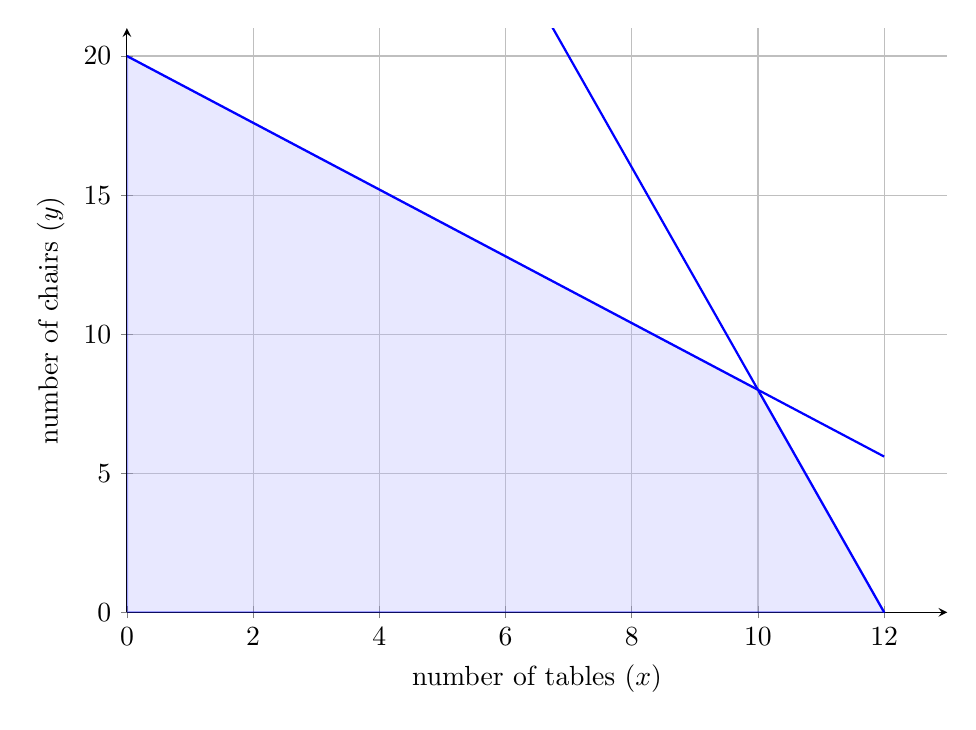
\begin{tikzpicture}
  \begin{axis}[
    xlabel={number of tables ($x$)},
    ylabel={number of chairs ($y$)},
    axis lines=left,
    xmin=0, xmax=13,
    ymin=0, ymax=21,
    xtick={0,2,4,6,8,10,12},
    ytick={0,5,10,15,20},
    width=12cm,
    height=9cm,
    grid=both,
    enlargelimits=false,
  ]

  % Feasible region (blue fill)
  \addplot[fill=blue!30, draw=blue, opacity = 0.3, thick] coordinates {
    (0,0)
    (0,20)
    (10,8)
    (12,0)
    (0,0)
  };

  % Constraint lines
  \addplot[domain=0:12, thick, blue] {48 - 4*x}; % 80x + 20y = 960
  \addplot[domain=0:12, thick, blue] {20 - 1.2*x}; % 12x + 10y = 200

  % Integer points in feasible region (commented out)
%  \foreach \pt in {
%    (0,0), (0,20), (10,8), (12,0),
%    (1,18), (2,16), (3,14), (4,12), (5,10), (6,8), (7,6), (8,4), (9,2), (10,0)
%  } {
%    \addplot[only marks, mark=*, mark size=2pt, black] coordinates {\pt};
%  }

  \end{axis}
\end{tikzpicture}
\end{document}
